\pdfoutput=1

\documentclass{l4proj}

%
% put any packages here
%

\usepackage[]{algorithm2e}
\usepackage{graphicx}
\graphicspath{ {images/} }

\begin{document}
\title{Who's There? Occupancy Prediction with Smart Sensor Boxes}
\author{Jamie Sweeney}
\date{September 26, 2017}
\maketitle

\begin{abstract}
We show how to produce a level 4 project report using latex and pdflatex using the 
style file l4proj.cls
\end{abstract}

\educationalconsent
%
%NOTE: if you include the educationalconsent (above) and your project is graded an A then
%      it may be entered in the CS Hall of Fame
%
\tableofcontents
%==============================================================================


%==============================================================================
\chapter{Introduction}
\pagenumbering{arabic}


\section{Context}
The “internet of things”, or the IoT is a term used to describe a wide network of connected devices, ranging from supercomputers to “smart appliances”. Since the term was first coined in 1999 [1], the IoT has come a long way with new applications being discovered consistently [source needed], with a predicted market of £6.5 trillion) by 2020 \cite{test}.

One key area of study has been developing occupation detection that would allow IoT devices to be more aware of the occupation status of their surroundings. This is a crucial step to implementing smart homes, workplaces and campuses that are responsive and can meet their demands at any given time.

Advanced examples are already taking form, with the University of Glasgow investing €1bn towards developing a smart campus and the city of Barcelona making major overhauls to many public services in an attempt to bring the idea of a smart city to reality.
Goals
The aim of this project is to design and construct low budget ‘smart sensor boxes’, capable of predicting human occupation in a room. To do this we use the popular brand of microprocessors ‘Raspberry Pis’ in addition to a variety of sensors and other techniques.

In addition to the smart sensor boxes, we will design and implement a centralised hub capable of receiving, storing and serving information produced by a series of RPi boxes. This hub should also provide functionality for system-wide maintenance and configuration, to make setup and operation efficient and flexible.


\section{Motivations}
The motivations for this project are wide, with smart sensors being applicable in a broad variety of ways. We will discuss the primary motivations for this project, which are understandably more relatable and accessible to myself, in addition to a number of secondary motivations that are considered due to close similarity.

\subsection{Primary Motivation}
To narrow our field of focus, we choose a main motivation to consider when producing the smart sensor boxes. We consider the following scenario: University administration decide they wish to upgrade buildings with ‘smart sensor boxes’ with the overall goal being that student or other staff member can find current/past occupancy information on certain areas remotely. For example library group study areas could be listed online with an indication of their current use, allowing students who plan on visiting to check availability beforehand.
The University of Glasgow library currently provides a similar feature, displaying computer use breakdown by floor, available from monitors within the library.

In addition the system should be built to be easily extendable, and capable of operating as a part of a larger IoT network.

\subsection{Secondary Motivations}
Although we focus on a university implementation of occupancy prediction, we can imagine a similar design could be incorporated into many different areas. Schools, workplaces and public buildings could benefit from installing smart sensor functionality, allowing not only occupancy information to the user, but also providing more in-depth analysis of overall occupation to any interested administrators.

An example of this would be public buildings that allow local councils to analyse the usage of public service, allowing them to make more informed decisions on funding, maintenance, staffing and other key elements of successful operation.

Smart sensor data would come in useful for many other functions, perhaps one of the most useful being used as supplementary information to existing systems. For example automated heating, ventilation, lighting and other system functions could benefit from the additional knowledge and perhaps function more independently as a result.

To list a few more: Security systems, home-automation, public transport, gyms, dining locations and other areas of leisure.



%==============================================================================
\chapter{Background Analysis}
We start by researching and reviewing past studies conducted in similar fields, given that the subject matter is broad and widely applicable, we find many studies available. Many employing sensors 


\section{Sensor Research}
Sensors are a key element in almost every real-world computing application, especially those concerned with the detection of humans e.g automatic doors. Without them a computing device would have little to no information on its surroundings, and would be extremely ineffective. For this reason, sensors will be a primary component of the smart boxes.

Background research on previously conducted studies gives us a comprehensive list of applicable sensor, and their specific advantages and disadvantages.

\subsection{Passive Infrared Sensors}
Infrared light is the electromagnetic radiation emitted by all objects with a temperature above 0°K, giving the feeling of heat. The wavelength of IR light spans from 700 nm to 1 mm, existing just outside of the range of human vision. PIR sensors feature a “sensor face” that can detect a change in the average amount of IR light hitting the surface, the sensor then outputs a signal indicating this change, with a low voltage indicating low change, and a higher voltage indicating a greater change.

They are most commonly used in PIR-based motion detectors such as automatic lighting systems. Generally the purpose of a PIR sensor is to detect the presence of humans at a binary level i.e true or false. However it has been shown that with suitable positioning and utilisation of machine learning techniques, a PIR sensor can be used to predict the number of occupants in a room within a small range to fair accuracy.

There are many problems to overcome when using a PIR sensor for this purpose, most importantly, the positioning of the sensor; PIR sensors are prone to interference from occluding objects i.e blocking one another from the sensor. As a result of this, the most ideal position would be the ceiling of the room, however this may not prove as practical for other aspects of performance.

Although it will be impossible to obtain a precise estimation by a PIR sensor alone, with the correct implementation, the sensor could be used alongside other components to provide a valid prediction.

\subsection{Image / Video}

\subsection{Audio}

\subsection{Other}


%==============================================================================
\chapter{Requirements}

\section{Functional Requirements}

\subsection{Sensor data collection}
The smart sensor boxes should be capable of collecting data from connected sensors for a specified period of time. The connected sensors we should support are:
\begin{enumerate}
  \item Bluetooth device scanning.
  \item Bluetooth Low Energy device scanning.
  \item Camera
\end{enumerate}
However the final system should be easily extendible so that new sensors can be added without too much cost.

\subsection{Reporting}
The smart sensor boxes should be capable of and able to report this data periodically to a centralised storage location.

\subsection{Estimation}
The system should be able to analyse these "Smart Box" reports, to give an estimation of occupancy for each location with reports.

In order to improve the estimation results, there should be some way of manual readings to be submitted and stored.

\subsection{Data serving}
The report data produced should be made available to authorised users and applications.
The estimations produced should be made available to any potential end users and applications.

In addition, authorised users should be able to insert new, delete or amend information on:
\begin{itemize}  
  \item Buildings, floors, rooms.
  \item Smart boxes.
  \item Admin users.
\end{itemize}

\subsection{Data storage}
The system must be capable of storing data about: 
\begin{enumerate}
  \item Buildings, floors, rooms.
  \item Smart boxes.
  \item Sensor output.
  \item Smart box reports.
  \item Estimations.
  \item Manual readings
  \item Admin users.
\end{enumerate}

\section{Non-functional Requirements}
\subsection{Sensor data collection}
\begin{itemize}
  \item Ideally each smart sensor box should be as cheap as possible while providing adequte data, in order for the system to be scaled up without large overhead costs.
  \item For each sensor method, if the data can be collected continuously i.e results can be streamed in real time, then it should be done so with as little downtime as possible. If the data cannot be collected continuously, meaning they require some amount of time to compute results before obtaining a new reading, then we should perform as many iterations as possible to ensure that results are up to date.
  \item The data collection should be able to run for as long as possible without human intervention to reduce the amount of maintainence required.
\end{itemize}

\subsection{Reporting}
\begin{itemize}	
  \item To ensure that occupancy reports and predictions are not outdated, RPis should be able to send reports at a rate of atleast one report per minute. The reports should also stick to the specified rate with fair accuracy and not deviate too far from a steady report rate.
  \item To prevent irregularities in the sensor data affecting reports, the reports should use some form of smoothing mechanism, which would cause any sudden changes in sensor readings to have a smaller effect on the overall estimate.
  \item Report structure should allow for partial reports from sensor boxes not equipped with all sensors, and also allow for easy extensibility to allow for new sensor additions.
  \item Report structure should take a common format such as JSON.
\end{itemize}

\subsection{Estimation}
\begin{itemize}	
  \item The estimates should be as accurate as possible.
  \item Estimates should be produced at a reasonable enough rate to ensure that they are not out of date.
\end{itemize}

\subsection{Data serving}
All data served to users should be:
\begin{itemize}	
  \item In a user-friendly and informative format.
  \item As close to real time as possible.
  \item Data 

\end{itemize}

\subsection{Data storage}
Any data stored should:
\begin{itemize}	
  \item Be implemented in an efficient and correct manner, without unnecessary dependencies between data.
  \item Easily scaleable without any major modifications.
  \item Accessible as quickly as possible and with no down-time.
  \item Secure from malicious attack or unauthorised access.
\end{itemize}



%==============================================================================
\chapter{Design}
\section{High Level Summary}

We start by splitting the requirements to three seperate components with individual functions.
\begin{enumerate}
  \item Smart Sensor Boxes:
	Collects data from the various sensors, also generate reports detailing RPi identification, allong with smoothed sensor data. Reports are then sent to the HTTP server for analysis. 
  \item Centralised Storage:
	A database that allows for the storing and querying of data must contain information on building, RPis, estimates, reports, users etc.
  \item HTTP Server:
	A simple HTTP application that can receive sensor report data from the smart sensor boxes. The sever should also be able to perform estimations for locations based on reports and also feature a web application that serves this data to the users. 
\end{enumerate}
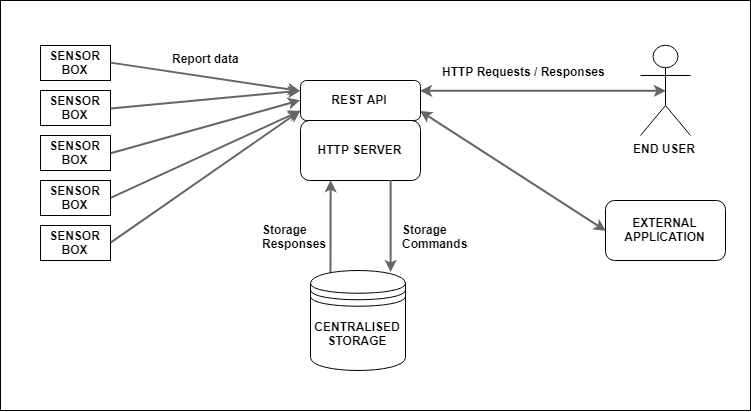
\includegraphics[width=\textwidth]{overalldiag}


\section{Components}
\subsection{Smart Sensor Boxes}
The smart sensor box logic consist of a main reporter algorithm which initialises scanning for each detection method and monitors the output. Every time a report is required, the algorithm takes the outputs from each output queue, and collates them to a report which is sent to the HTTP server for furthur use.  Algorithm \ref{RPA} shows the pseudocode for this algorithm.

The detection methods supported are:
\begin{enumerate}
  \item Bluetooth / BTLE device scanning -  Continuously scans for devices and adds any discoveries to a output map, scans are done for a specified time before restarting to ensure that devices do not stop responding the the scan signal. Algorithm \ref{BTS} details the algorithms used.
  \item Camera and object detection -  Runs on a loop taking images and feeding them into an object detection algorithm which predicts objects and their certainty. The number of people is extracted from the detection output and smoothed with previous results using an average of the previous value and the new prediction. Algorithm \ref{CMS} details the algorithms used.
\end{enumerate}



\begin{algorithm}
\DontPrintSemicolon
\nl $\textbf{void}~scanBluetooth(\textbf{Int}~T_{cycle}, \textbf{Int}~T_{timeout}, \textbf{Int}~T_{decay}, \textbf{Map}~output)$ \;
\nl \Begin{
\nl \While {$T_{timeout} > T_{now}$}{
\nl $scan(T_{cycle}, T_{decay})$\;
\nl \While {$scanning$}{
\nl $discovery \gets new\textunderscore discovery$\;
\nl $handleDiscovery(T_{decay}, discovery, output)$\;
}
}
}
\;

\nl $\textbf{void}~scanBluetoothLowEnergy(\textbf{Int}~T_{cycle}, \textbf{Int}~T_{timeout}, \textbf{Int}~T_{decay}, \textbf{Map}~output)$ \;
\nl \Begin{
\nl \While {$T_{timeout} > T_{now}$}{
\nl $scan(T_{cycle}, T_{decay})$\;
\nl \While {$scanning$}{
\nl $discovery \gets new\textunderscore discovery$\;
\nl $handleDiscovery(T_{decay}, discovery, output)$\;
}
}
}
\;

\nl $\textbf{void}~handleDiscovery(\textbf{Int}~T_{decay}, \textbf{Map}~discovery, \textbf{Map}~output)$ \;
\nl \Begin{
\nl $addr \gets discovery['address']$\;
\nl $rssi \gets discovery['rssi']$\;
\nl $time \gets discovery['time']$\;
\nl \eIf {$address\ in\ output$}{
\nl $old \gets output[addr]$\;
\nl \eIf {$old['time'] + T_{decay} < T_{now} $}{
\nl $new \gets \{'rssi': (rssi + old['rssi'])/2, 'time': time\}$\;
\nl $output[addr] \gets new$\;
\nl }{
\nl $new \gets \{'rssi': rssi, 'time': time\}$\;
\nl $output[addr] \gets new$\;
}
}{
\nl $new \gets \{'rssi': rssi, 'time': time\}$\;
\nl $output[addr] \gets new$\;
}
}
\;
\caption{Pseudocode for Bluetooth and Bluetooth Low Energy device scanners.}
\label{BTS}
\end{algorithm}

\begin{algorithm}
\DontPrintSemicolon
\nl $\textbf{void}~scanCamera(\textbf{Int}~T_{cycle}, \textbf{Int}~T_{timeout}, \textbf{Int}~output)$ \;
\nl \Begin{
\nl \While {$T_{timeout} > T_{now}$}{
\nl $img \gets takeImage()$\;
\nl $objs \gets objectDetection(img)$\;
\nl $hum \gets numHuman(objs)$\;
\nl $output \gets (output + hum)/2$\;
\nl $wait(T_{cycle})$\;
}
}
\;
\caption{Pseudocode for the camera detection algorithm.}
\label{CMS}
\end{algorithm}

\begin{algorithm}
\DontPrintSemicolon
\nl $\textbf{void}~reporter(\textbf{Int}~T_{cycle}, \textbf{Int}~T_{timeout})$ \;
\nl \Begin{

\nl $T_{decay}, T_{ccycle}, T_{bcycle} \gets getConfig()$\;

\nl $bt\textunderscore output \gets new\ \textbf{Map}$\;
\nl $cm\textunderscore output \gets 0$\;

\nl $scanBluetooth(T_{bcycle}, T_{timeout}, T_{decay},bt\textunderscore output)$\;
\nl $scanBluetoothLowEnergy(T_{bcycle}, T_{timeout}, T_{decay},bt\textunderscore output)$\;
\nl $scanCamera(T_{ccycle},T_{timeout}, cm\textunderscore output)$\;

\nl \While {$T_{timeout} > T_{now}$}{

\nl $devices \gets bt\textunderscore output$\;
\nl $people \gets cm\textunderscore output$\;
\nl $report \gets \{ 'devices':devices, 'people':people, 'time': T_{now}'\}$\;
\nl $sendReport(report)$\;
\nl $wait(T_{cycle})$\;
}
}
\;

\caption{Pseudocode for the reporter algorithm.}
\label{RPA}
\end{algorithm}


\subsection{Centralised Storage}
\subsection{HTTP Server}





%==============================================================================
\chapter{Implementation}


\section{High Level Summary}
\section{Components}
\subsection{Smart Sensor Boxes}
\subsection{Centralised Storage}
\subsection{HTTP Server}


%==============================================================================
\chapter{Evaluation}



%==============================================================================
\chapter{Conclusion}
\section{Summary}
\section{Future Work}
\section{Reflection}


%%%%%%%%%%%%%%%%
%              %
%  APPENDICES  %
%              %
%%%%%%%%%%%%%%%%
\begin{appendices}

\chapter{Title of appendix}
Put some data in here:
\begin{verbatim}
      > blahblahblah
\end{verbatim}

\end{appendices}

%%%%%%%%%%%%%%%%%%%%
%   BIBLIOGRAPHY   %
%%%%%%%%%%%%%%%%%%%%

\bibliographystyle{plain}
\bibliography{bib}

\end{document}
